\documentclass{article}
\usepackage{ngerman}
\usepackage[utf8]{inputenc}
\usepackage{graphicx} 
\usepackage[hyperfootnotes=false]{hyperref}
\hypersetup{colorlinks,linkcolor=blue} 



\title{Projektmanagment und Teamarbeit\\Klasse 5IA, TFO Bozen\thanks{Erstellt 
im Kurs ``Projektmanagment und Betriebsorganisation'', TFO Bozen, Mai 2015. Lehrkraft: Mirko Morandini}}

\author{Berger Dominik
\and Bernard Simon
\and Dalvai Ragnioli Peter
\and Baron von Treuheim Stefan Maximilian Di Pauli
\and Domaneg Andreas
\and Gobbi Viktor
\and Hopfgartner Christopher
\and Mussner Marcel
\and Niederegger Andreas
\and Niedrist Alexander
\and Nocker Thomas
\and Oberprantacher Hannes
\and Pirpamer Damian
\and Pazeller Daniel
\and Prader Matthias
\and Rassele Phillip
\and Romen Ren\'e 
\and Rizzolli Thomas
\and Rufinatscha Samuel}


\begin{document}

\maketitle


\begin{abstract}
Die folgende Arbeit besch"aftigt sich mit verschiedensten Programmen zum Thema ``Projektmanagement und Teamarbeit''.
Software und Online-Services aus verschiedenen Bereichen werden vorgestellt, die die Zusammenarbeit im Team und im Betrieb unterst"utzen: Versionskontrolle, Issue-Tracking, Build-Management, Kommunikation, Konfigurations-Management, Workflow Management, Enterprise Resource Planning und Project-Management.

Jeder Sch"uler hatte die Aufgabe, sich "uber eine Software zu informieren, einen Vortrag zu gestalten und eine Latex-Datei mit einer Zusammenfassung zu formulieren. 
\end{abstract}

\newpage


\begin{sloppypar}
\tableofcontents
\listoffigures

\newpage
\section{SVN}
\subsection{Allgemeines  \"uber Subversion (SVN)}
Apache Subversion (kurz: SVN) ist eine Software zur Versionsverwaltung von Dateien und Verzeichnissen. Es ist ein zentrales Verwaltungssystem. SVN ist unter der Apache-Lizenz 2.0 ver\"offentlicht und somit Open-Source. Bei SVN erfolgt die Versionierung \"uber ein zentrales Repository. Bei einer Ver\"anderung einer Datei oder eines Verzeichnisses werden zwischen dem Repository und dem Arbeitsplatz nur die Unterschiede \"ubertragen. Merkmale eines zentralen Verwaltungssystemes:
\begin{itemize}
    \item Es gibt nur eines Server aber mehrere Workingcopies
    \item Versionsnummern werden zentral vergeben
    \item Versionshistorie ist nur auf dem Server gespeichert
    \item erm\"oglicht Zugriffs- und Rechtemanagement
\end{itemize}

\begin{figure}[h!]
\centering

\includegraphics[width=\textwidth]{subversion_logo.png}
\caption{Subversion Logo}
\label{fig:SVlogo}
\end{figure}

\subsection{Geschichtlicher Hintergrund}
SVN entstand im Jahre 2000 im amerikanischen Unternehmen CollabNet.
Im November 2009 entschloss CollabNet, dass das Projekt (SVN) an die Apache Software Foundation geht. Danach wurde das Projekt von Apache zu Apache Subversion unbenannt.

\subsection{Vorteile gegen\"uber CVS}
\begin{description}
\item[Die wichtigsten Vorteile]~\par
   \begin{itemize}
      \item Versionsschema
      \begin{itemize}
         \item CVS kann nur die Versionsgeschichte von einzelnen Dateien speichern. SVN von Dateien und Verzeichnissen
      \end{itemize}
      \item \"Anderungsverfolgung
        \begin{itemize}
         \item CVS muss bei einer \"Anderung immer die gesamte Datei \"ubertragen
      \end{itemize}
      \item Umbenennungen und Verschiebungen
              \begin{itemize}
         \item Bei einer Umbenennung oder Verschiebung einer Datei wird in CVS die gesamte Versionsgeschichte gel\"oscht
      \end{itemize}
      \item L\"oschmarkierung von Verzeichnissen
              \begin{itemize}
         \item In CVS k\"onnen nur leere Verzeichnisse gel\"oscht werden
      \end{itemize}
   \end{itemize}
\end{description}
 
 \subsection{Vorteile gegen\"uber GIT}
\begin{description}
\item[Die wichtigsten Vorteile]~\par
   \begin{itemize}
      \item Kostenfrei
      \item Sehr gut getestet
      \item Sehr aktuell, da es stetig weiterentwickelt wird von Apache
      \item Sehr gute Unterst\"utzung von IDE's und Shared Hosting Anbietern (z.B. SourceForge)
         \item Einfache Handhabung
   \end{itemize}
\end{description}
 
\subsection{Die Architektur von Subversion}
Subversion ist auf einem Client-Server-Modell aufgebaut. Auf dem Computer des Benutzers wird ein Client ausgef\"uhrt. Dieser kann \"uber verschiedene Verbindungsarten auf den Server zugreifen. Die ganzen Information \"uber Dateien (Informationen \"uber Zust\"ande, Versionen, Kommentare) und die Dateien selbst liegen auf dem Server. Das Repository selbst, welches auf dem Server liegt, kann entweder in einer BerkleyDB-Datenbank oder direkt auf dem Dateisystem gespeichert werden. Derzeit gibt es drei Zugriffsvarianten:
\begin{itemize}
    \item HTTP / HTTPS
    \item SVN (subversioneigenes \"Ubertragungsprotokoll)
    \item FILE (lokaler Zugriff)
\end{itemize}
\newpage
\begin{figure}[!htbp]
\centering
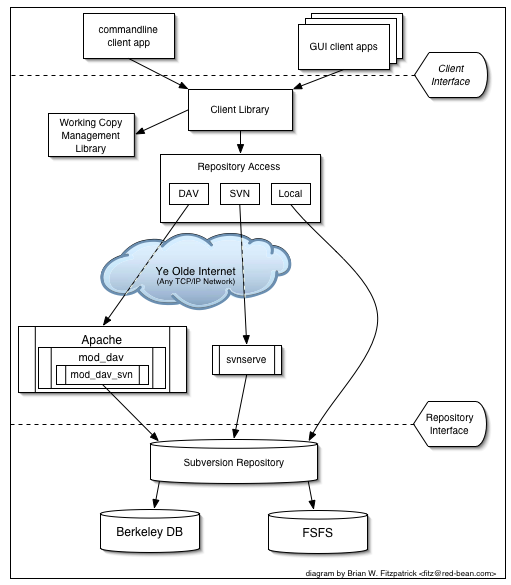
\includegraphics[height=15cm]{subversion_architektur.png}
\caption{Subversion Architektur}
\label{fig:SVarch}
\end{figure}

\subsection{Die Komponenten von Subversion}
Subversion besteht aus verschiedenen Softwareteilen:
\begin{itemize}
    \item svn
        \begin{itemize}
            \item Kommandozeilenprogramm
        \end{itemize}
    \item svnversion
        \begin{itemize}
            \item Schreibt die Revisionsnummer der Arbeitskopie in die Standartausgabe
        \end{itemize}
    \item svnlook
        \begin{itemize}
            \item Werkzeug um ein Projektarchiv zu untersuchen
        \end{itemize}
    \item svnadmin
        \begin{itemize}
            \item Werkzeug um ein Projektarchiv zu erstellen, zu ver\"andern oder zu reparieren
        \end{itemize}
    \item mod\_dav\_svn
        \begin{itemize}
            \item Plugin f\"ur den Apache-HTTP Server um ein Projektarchiv  \"uber ein Netzwerk verf\"ugbar zu machen
        \end{itemize}
    \item svnserve
        \begin{itemize}
            \item Serverprogramm; Andere M\"oglichkeit um Projektarchiv \"uber ein Netzwerk verf\"ugbar zu machen (SSH)
        \end{itemize}
    \item svnsync
        \begin{itemize}
            \item Tool, um Revisionen eines Projektarchivs in ein anderes Projektarchiv zu \"uberspielen.
        \end{itemize}
\end{itemize}

\subsection{Begriffe in SVN}
\begin{description}
\item[Bei Subversion sind folgende Begriffe wichtig:]~\par
   \begin{itemize}
        \item Revision
        \item Changeset
            \begin{itemize}
        \item Ein Changeset ist eine Zusammenfassung aller \"Anderungen einer Version. Bei einem Changeset gibt es folgende Notations:
        \begin{itemize}
        \item U = Updated
        \item D = Deleted
        \item A = Added
      \end{itemize}
      \end{itemize}
      \item Delta / Diff
              \begin{itemize}
         \item Unter Delta / Diff versteht man die Differenzen zwischen zwei Versionen. In SVN werden immer nur die Unterschieden zwischen zwei Versionen festgehalten.
      \end{itemize}
      \item Merge
              \begin{itemize}
         \item Unter Merge versteht man das Zusammenf\"uhren von verschiedenen \"Anderungen in zwei Versionen einer Datei.
      \end{itemize}
       \item Branch
              \begin{itemize}
         \item Ein Branch ist eine Kopie einer Ursprungsversion.
      \end{itemize}
       \item Tag
              \begin{itemize}
         \item Mit einem Tag kann man die einzelnen Versionen beschriften.
      \end{itemize}
   \end{itemize}
\end{description}
 
 \subsection{Terminal - Befehle f\"ur SVN}
 \begin{description}
\item[Neuen Baum auf den lokalen Rechner kopieren:]~\par
   \begin{itemize}
      \item svn checkout [Pfad] [Lokaler Name]
   \end{itemize}
\item[Lokalen Baum aktualisieren:]~\par
   \begin{itemize}
      \item svn update
   \end{itemize}
\item[Lokale Dateien hinzuf\"ugen und l\"oschen:]~\par
   \begin{itemize}
      \item svn add file...
      \item svn remove file...
   \end{itemize}
   \item[\"Ubersicht \"uber lokale \"Anderungen:]~\par
   \begin{itemize}
      \item svn status
   \end{itemize}
      \item[Lokale \"Anderungen ins Repository \"ubertragen:]~\par
   \begin{itemize}
      \item svn commit -m "Beschreibung der Änderungen"~\par
   \end{itemize}
\end{description}

\subsection{Ist SVN noch aktuell?}
SVN wird durchaus auch heutzutage noch verwendet. Jedoch ist seine gr\"o"ste Konkurrenz GIT, welches mittlerweile weiter verbreitet ist. Es gibt aber einen gro"sen Unterschied zwischen GIT und SVN: GIT ist dezentralisiert und SVN zentralisiert. Deshalb wird SVN auch nicht so schnell verschwinden, da beide Systeme ihr Vor- und Nachteile haben.
\section{Trello}
Trello ist eine web-basierte Projektmanagementsoftware. Diese Software wurde von US-amerikanischen Unternehmen Fog Creek Software entwickelt. Trello nutzt MongoDB, Node.js und Backbone.js. Dieses Projekt wurde mit JavaScript verwirklicht.

\begin{figure}[h]
  \centering
    
\includegraphics[width=\textwidth]{trello.png}
  \caption{Logo von Trello}
  \label{fig:trello}
\end{figure}
\subsection{Geschäftsmodell}
Geschäftsmodell von Trello basiert auf dem Freemium-Prinzip: Die Grundfunktionen sind kostenlos verfügbar. Jedoch Extrafunktionen können nur mit einen Gold-Account genutzt werden.
\subsection{Geschichte}
Im Sommer 2010 beginnt Fog Creek Software mit einem potenziellen Produkt her zum zu entwickeln. Im Januar 2011 wird ein Prototyp vorgeschlagen, der zur Lösung einiger hochrangiger Planungsprobleme dienen soll. Sein Name lautet Trellis. Kurz danach beginnt die Entwicklung in Vollzeit.

Nach abgeschlossener Betaphase startet Trello im September 2011 auf der TechCrunch Disrupt mit Apps für Internet und iPhone. Ab hier wurde der Name Trell gewählt.

Der Dienst wurde am 13. September 2011 gegründet und ist nur in English verfügbar. Aktuell hat Trello 7 Millionen Benutzer (Stand: Januar 2015). Der Entwichlung dieses Dienstes fand nach dem Vorbild der Produktionsplanungsmethode Kanban statt. Dies kann über ihre Webanwendung trello.com oder über ihre App die für iOS, Android und Windows 8 verfügbar ist.

Im Sommer 2012 wurde Taco, der Husky von Fog Creek-Mitbegründer Joel Spolsky, Maskottchen von Trello. Trello erreicht die Marke von 500.000 Mitgliedern und führt die Trello-Android-App ein.
\begin{figure}[h]
  \centering
    
\includegraphics[width=0.7\textwidth]{taco.png}
  \caption{Maskottchen Taco}
  \label{fig:taco}
\end{figure}
\subsection{Nutzung}
Ihr Dienst läuft über ihre sogenannten Boards. Hier können Listen bearbeitet und modifiziert werden. Es können Checklisten, Anhänge und mit einem festgelegten Termin versehen werden. Den Zugriff auf diese sogenannten Boards kann beliebig vielen Nutzern zur Verfügung gestellt werden. Dies kann durch ein einfaches Drag and Drop gemacht werden. Diese können sich bei der Planung und der Kommunikation des Projekts beteiligen. Hier können an die Bretter verschiedene Probleme angesprochen und zusammen gelöst werden. Der Dienst bietet den Nutzern die Möglichkeit Kommentare zu hinterlassen, Dateien hochzuladen, Checklisten erstellen, Termine und viele weitere Features.
Daten können nicht nur vom Computer selbst sondern acuh von Google Drive, Droppbox oder OneDrive hinzugefügt werden. Um das ganze noch aufzupeppen sind \glqq emojis\grqq \space auch natürlich verfügbar. Um auf den laufenden über sein Projekt zu sein Wird man in der App selbst benachrichtigt, über E-Mail, Desktop Benachrichtigungen über den Browser oder über \glqq push notifications\grqq.

Hier ein kleines Video dazu: https://goo.gl/ehSahR


\documentclass[a4paper, 11pt]{article} 
\usepackage[ngerman]{babel} 
\usepackage[ansinew]{inputenc} 
\usepackage{graphicx} 
\usepackage{caption}
\usepackage{subcaption}
\usepackage{float}
\usepackage{url}
\usepackage{lipsum}
\usepackage{calc}
\usepackage{pgf-umlsd}

\begin{document}
\begin{center}
Bonita BPM
\end{center}
\newpage
\tableofcontents
\newpage
\section{Was ist Bonita BPM?}
Bonita PBM ist eine Open Source Software Suite f�r Prozessmodellierung,  Gesch�ftsprozessmanagement (BPM) und Arbeitsablaufverwaltung (Workflow-Engine).  Damit ist es m�glich Prozesse zu automatisieren, dern Ergebnisse zu messen und diese Prozesse anschlie�ens zu verbessern. Die Suite besteht aus 3 Teilen: 
\begin{itemize}
 \item{\textit{Bonita Studio}: ein Studio in dem der Benutzer die Gesch�ftsprozesse grafisch bearbeiten kann. Im Studio kann auch die vom Web aus erreichbare Gesch�ftsanwendung generiert werden. Eine weitere Funktion des Bonita Studios ist es die Gesch�ftsprozesse mit anderen Standards und Technologien zu designen.}
 \item{\textit{Bonita Portal}: ein Protal das dem Endbenutzer und den Administratoren mittels seiner Webseite eine �bersicht �ber die Aufgaben und Prozessse zur Verf�gung stellt.}
 \item{\textit{Bonita Execution Engine}: eine Java Engine um programmiertechnisch mit den Prozessen zu interagieren}
\end{itemize}

\section{Wer braucht BonitaBPM?}
\begin{itemize}
\item{\textit{Angestellte:} Mit Bonita BPM haben Angestellte einen �berblick dar�ber, welche Arbeiten anstehen und in welcher Reihenfolge diese abzuarbeiten sind.}
\item{\textit{Teamchefs:} Mit der Hilfe von Bonita BPM k�nnen Teamchefs Aufgaben auf ihr Team verteilen.}
\item{\textit{Manager:} Durch die Aktivit�tsanalyse die mit Hilfe von Diagrammen erstellt werden kann, k�nnen Manager die Produktivit�t der Firma erh�hen.}
\end{itemize}
\section{Funktionalit�ten}
Bonita BPM bringt verschiedene Funktionen um das Gesch�ftsprozessmanagement (BPM) von Projekten zu planen, zu entwickeln, ausf�hren und zu �berwachen:
\begin{itemize}
 \item{\textit{Live Updates der Prozesse}: Neue Versionen von Prozessen k�nnen in der Produnktionsumgebung einfach aktualisiert werden}
 \item{\textit{Versionskontrolle der Prozesse}: W�hrend der modellierung der Prozesse k�nnen verscheidene provisorische Versionen der Prozesse gespeichert und verwaltet werden}
 \item{\textit{Simulation der Prozesse}: Bonita BPM bietet die M�glichkeit dir Prozesse mit verschiedenen Parametern wie Kosten, Dauer, Ressourcenkonsum usw. zu simulieren.}
\item{\textit{Zuweisen und filtern von Aktivit�ten}: Mit den eingebauten Instrumenten und Filtern ist es m�glich einer oder mehrerer Personen dynamisch und effizient Aktivit�ten zuzuweisen.}
\item{\textit{Zentrales Repository}: Im zentralen Firmenrepository ist es m�glich alle Prozesse zu speichern, organisieren und archivieren}
\end{itemize}
\section{Weitere Eigenschaften}
Bonita BPM macht es m�glich das Gesch�ftsprozessmanagement mit weiteren Bereichen eines Unternehmens zu verbinden. Zum Beispiel mit dem Kundenbeziehungsmanagement oder dem Ressourcenplanungsmanagement. Des weiteren bietet die Software Suite einen Kommentarfeed zu jedem spezifischen Fall um die Kommunikation innerhalb des Unternehmnens zu f�rdern. Bonita BPM steht in den Sprachen Englisch, Franz�sich und Spanisch zur Verf�gung. Die Interfaces k�nnen durch ein eigenes Werkzeug aber in jede beliebige Sprache �bersetzt werden. Es ist weiters m�glich Prozesse in Echtzeit zu �ndern oder diese zu analysieren.
\end{document}
\documentclass{article}
\usepackage[utf8]{inputenc}

\title{DokuWiki}
\author{Philipp Rassele}
\date{\today}

\begin{document}

\maketitle

\section{DokuWiki}
\subsection{Was ist DokuWiki?}
DokuWiki ist eine freie Wiki-Software,die in der Programmiersprache PHP geschrieben und unter der GPL 2 lizenziert wurde. Dokuwiki wurde von Andreas Gohr 2004 ins Leben gerufen. Um Inhalte und Metadaten zu speichern, werden einfache Textdateien genutzt und keine SQL-Datenbanken, wie bei anderen Wiki-Engines. Um die Wikiquellseiten gut leserlich zu halten, werden Inhalt und Metadaten von Wikiseiten bei DokuWiki strikt getrennt. Anfangs zur einfachen Dokumentation von Projekten gedacht, wird Dokuwiki mittlerweile aufgrund seiner Einfachheit und Funktionen für eine Vielzahl von Anwendungen eingesetzt. Auf Basis einer übersichtlichen Struktur lassen sich mit Erweiterungen (Plugins) weitere Funktionen hinzufügen, etwa für Blogs, Mediendaten oder Arbeitsgruppen.
\subsection{Merkmale}
\subsubsection{Versionsverwaltung}
Die Versionverwaltung speichert alle Versionen einer Wikiseite. Es ist möglich, ältere Versionen mit der aktuellen Version zu vergleichen. Außerdem wird verhindert, dass mehrere Benutzer gleichzeitig eine Seite verändern können.
\subsubsection{Zugriffskontrolle}
Die Zugriffsrechte lassen sich für Kombinationen von Benutzern, Gruppen und Namespaces vergeben. Die Einstellung ist via Webinterface (Usermanager) oder manuell per Konfigurationsdatei möglich (Access Control List).
\subsubsection{Add-ons}
DokuWiki hat einen einfachen Add-on-Mechanismus.Dadurch ist es möglich Erweiterungen (Plugins) in PHP zu schreiben. Es gibt inzwischen eine ganze Reihe an Erweiterungen (>300). Über den Plug-in-Manager können diese über die Web-Oberfläche in das eigene Wiki integriert und verwaltet werden.
\subsubsection{Templates}
Das Aussehen des Wikis kann der Administrator über Templates festlegen. Es wurden inzwischen unterschiedliche Templates von der Entwicklergemeinde zur Verfügung gestellt.
\subsubsection{Internationalisierung}
Als Standard-Zeichencodierung wird UTF-8 verwnedet. Somit sind auch Sprachen wie Chinesisch, Thai oder Hebräisch darstellbar. Das Wiki selber kann momentan in 39 Sprachen konfiguriert werden.
\subsubsection{Caching}
Um den Server des Wikis zu entlasten, speichert ein Cache geparste Seiten. Bei einem erneuten Aufruf der Seite werden die gespeicherten Daten geliefert, anstatt die Wikiseite nochmals zu parsen.
\subsubsection{Volltextsuche}
DokuWiki hat eine Volltextsuche integriert, mit der in dem gesamten Wiki nach Stichwörtern gesucht werden kann.
\subsubsection{WYSIWYG-Editor}
Der Wiki-Philosophie einer einfachen Markup-Syntax entsprechend hat DokuWiki in der Grundausstattung keinen WYSIWYG-Editor. Diese Funktion kann aber über ein Plugin nachgerüstet werden; alternativ gibt es eine Quickbuttonleiste ähnlich MediaWiki.
\subsubsection{Datenspeicherung}
DokuWiki speichert alle Daten (aktuelle und alte Seiteninhalte, Indizes, Caches) in Textdateien. Dadurch ist keine separat laufende Datenbank (etwa MySQL) notwendig.
\subsubsection{Versionierung/Synchronisation}
Jede Wiki-Seite wird in einer Textdatei im Verzeichnis dokuwiki-JJJJ-MM-TT/data/pages gespeichert, der Name der Datei bleibt trotz Versionierung gleich. Vorherige Versionen befinden sich unter dokuwiki-JJJJ-MM-TT/data/attic. Es erfolgt kein Umbenennen/Neuanlegen der Originaldatei (z. B. Revision00011, Revision00012). Dies macht Dokuwiki ideal für Synchronisations-Tools mit beidseitigem Abgleich und diff-Funktion wie Unison.
\subsubsection{Portable Version}
Für Windows-Rechner ist DokuWiki auch als portable Version zusammen mit einem portablen Apache Webserver für die Verwendung auf einem USB-Stick vorhanden.
\subsubsection{HTML5}
Seit Release 2012-10-13 ``Adora Belle'' parst DokuWiki HTML5-Seiten. 
\linebreak\linebreak 
Weitere Information über DokuWikie und \"ahnlicher Software findet man auf http://www.wikimatrix.org/.
\end{document}

\title{Gradle}
\author{Thomas Rizzolli}
\date{Mai 2015}

\maketitle

\section{Was ist Gradle}
Gradle ist ein Build-Management Tool wie Maven, dass in Java geschrieben wurde. Anders als Maven verwendet Gradle Groovie um die zu bauenden Projekte zu beschreiben. Im Gegensatz zu Maven, das XML verwendet, sind Gradle-Skripts direkt ausführbarer Code.

Gradle wurde für Builds von Projekten konzipiert, die aus einer Vielzahl von Unterprojekten besteht.
Da Builds umfangreicher Projekte sehr viel Zeit in Anspruch nehmen, unterstützt Gradle sowohl inkrementelles(st"uck f"ur st"uck) als auch Bauen der Software durch parallel ablaufende Build-Prozesse. Dadurch k"onnen nur Teile eines Projektes gebaut werden, die ge"andert wurden, ohne das Ganze Projekt neu bauen zu m"ussen. Des Weiteren k"onnen Tests parallel zum laufenden Build gestartet werden. Dadurch wird die Geschwindigkeit des Bauens des Projektes um ein Vielfaches erh"oht

Viele bekannte Frameworks verwenden Gradle, wie zum Beispiel Hibernate, Groovy, Grails und Spring Security. Auch Android ist seit Mitte 2013 hinzugekommen. Auch sogenannte ``nativer'' Systeme, welche nicht auf der Java-Plattform basieren, werden unterstützt. Dazu gehören die Programmiersprachen C++, C, Objective C und Assembler.

\section{Aufbau}
In Gradle braucht man in den meisten F"allen nur die build.gradle Datei. Gradle verf"ugt jedoch "Uber 2 weitere Dateien, die aber nicht unbedingt erforderlich sind.
\begin{itemize}
\item build.gradle - enth"allt die Definition der Tasks und der ganzen Abh"angigkeiten des Projektes
\item settings.gradle - hier werden die teilnehmenden Unterprojekte eines Multiprojekts definiert.
\item gradle.properties - enth"allt eine Liste von Eigenschaften f"ur eine projektspezifische Gradle-Initialisierung eines Builds
\end{itemize}

Weiteres wird in Gradle zwischen Tasks und Eigenschaften(Properties) unterschieden.

Tasks sind ausf"uhrbarer Code, der "uber die Kommandozeile aufgerufen wird, indem man dort ``gradle [den auszuf"uhrenden Task]'' eingibt.

Durch Properties werden die Eigenschaften des Builds, wie z.B. Pfad der Klassen und Abh"angigkeiten definiert werden. Eigenschaften k"onnen in zwei verschiedenen Weisen definiert werden:
\begin{enumerate}
\item \begin{verbatim}
sourceSets.main.java.srcDir "src/main/java"
\end{verbatim}
\item \begin{verbatim}
sourceSets{
    main{
        java{
            srcDir "src/main/java"
        }
    }
}
\end{verbatim}
\end{enumerate}
Beide Schreibweisen funktionieren, wobei meistens eine Kombination von 1. und 2. bevorzugt wird.
\section{Einfache Grundtasks}
Das Build-Script wird in der ``build.gradle'' geschrieben.

Zum Anfang ein einfaches Hello-World Programm:

In der build.gradle:

\begin{verbatim}
task helloworld {
    String hallo = 'Hallo'
    String welt = ' Welt!'
    println hallo + welt.toUpperCase()
}
\end{verbatim}

\section{Erstellen eines einfachen Java-Builds}
Wie bei den Tasks, werden auch Build-Scripts in der build.gradle definiert:

\begin{verbatim}
apply plugin: "java"

sourceSets {
    main.java.srcDir "src/main/java"
}

jar {
    manifest.attributes "Main-Class": "net.tfobz.test.Test"
}
\end{verbatim}
\begin{itemize}
\item Als erstes wird apply plugin: java gesetzt, damit Gradle mit Java-Projekten überhaupt umgehen kann.
\item Durch sourceSets.main.java.srcDir , kann der Pfad für die Java-Packages gesetzt werden. Wird diese Eigenschaft nicht gesetzt, dann wird standartm"asig ``src/main/java'' als Pfad gew"ahlt.
\item Die Eigenschaft jar.manifest.attributes erg"anzt die Manifest-Datei mit den gesetzten Attributen(in diesem Fall der Pfad der Main-Klasse).
\end{itemize}
\subsection{JUnit-Tests mit Gradle durchf"uhren}
Die Tests werden in Gradle, "ahnlich wie in Maven, getrennt vom Quellcode abgelegt. Standardm"a"sig ist der Pfad ``src/main/test'' eingestellt. Man kann diesen Pfad aber, wie es auch im vorherigen Beispiel gemacht wurde, "andern.

Folgendes Beispiel soll zeigen, wie man JUnit in seinem Projekt integrieren kann:
\begin{verbatim}
repositories {
    mavenCentral()
}

sourceSets {
    main.java.srcDir "src/main/java"
    test.java.srcDir "src/main/test"
}

dependencies {
    testCompile 'junit:junit:4.12'
}

test {
    testLogging {
        events 'started', 'passed', 'failed'
    }
}
\end{verbatim}
\begin{itemize}
\item Die Funktion mavenCentral() in der Eigenschaft repositories holt die erforderlichen Bibliotheken f"ur JUnit(Internetverbindung erforderlich).
\item In sourceSets.test.java.srcDir kann der Pfad der JUnit Testklassen ge"andert werden.
\item In der Eigenschaft testCompile in dependencies wird die zu verwendende JUnit-Version angegeben.
\item In der Eigenschaft test.testLogging.events werden die anzuzeigenden JUnit-Meldungen angegeben. Wird z.B. 'failed' weggelassen, so werden die gescheiterten JUnit-Tests nicht in der Konsole ausgegeben (Build schl"agt aber trotzdem fehl).
\end{itemize}

\subsection{Java Projekt eclipsf"ahig machen}
Um ein Gradle-Projekt eclipsf"ahig zu machen braucht man nur das Plugin ``eclipse'' hinzuzuf"ugen.
\begin{verbatim}
apply plugin: "java"
apply plugin: "eclipse"
\end{verbatim}

\begin{itemize}
\item Gibt man in der Kommandozeile den Befehl ``gradle eclipse'' ein, werden die ben"otigten Dateien f"ur Eclipse erzeugt. Das Projekt an sich wird aber weder compiliert noch getestet.
\item Mit dem Befehl ``gradle cleanEclipse'' werden die erzeugten Dateien wieder entfernt.
\end{itemize}

\documentclass[a4paper]{article}

\usepackage[english]{babel}
\usepackage[utf8x]{inputenc}
\usepackage{amsmath}
\usepackage{graphicx}
\usepackage[colorinlistoftodos]{todonotes}
\title{Microsoft Dynamics AX}
\author{Samuel Rufinatscha}

\begin{document}
\maketitle
\begin{sloppypar}

\section{Microsoft Dynamics AX}


\subsection{Einführung}
Microsoft Dynamics® AX ist eine objektorientierte ERP-Lösung von Microsoft® für mittelständische Unternehmen und Großunternehmen, die es ermöglicht, Wandel und Veränderungen aus dem Geschäftsumfeld aufzunehmen und mitzugestalten und so den Geschäftserfolg voranzutreiben. Es handelt sich um eine leistungsstarke Lösung, mit der man in kürzester Zeit einen nachhaltigen Nutzen erzielen kann.
Dank der 36 verfügbaren Landesversionen eignet sich die Software insbesondere für den Einsatz in multinationalen Organisationen.
Microsoft Dynamics AX 2012 stellt den Beginn eines neuen Produktivitätszeitalters bei Unternehmenslösungen dar. Es handelt sich um die neueste Version der erfolgreichen ERP Software Reihe und beeindruckt mit einem deutlichen Zuwachs an Funktionalität, einer völlig neuen Agilität und einer Benutzeroberfläche, die überzeugt und Produktivität beim Anwender fördert.


\subsection{Ausgangssituation zur Entwicklung der ERP Software}
Zur Entwicklung dieser ERP Software wurden relevante aktuelle Business und IT-Anforderungen einbezogen: steigender globaler Wettbewerb, verbunden mit signifikantem Kosten- und Preisdruck, Organisationsänderungen, aber Prozessoptimierungen, das Entstehen von komplexen internationalen Netzwerken oder erhöhte Anforderungen durch steigende gesetzliche Kontrolle sind wichtige Trends, der sich Unternehmen stellen müssen.Es wird absolute Transparenz für schnelle und richtige Entscheidungen gefordert.
Viele Organisationen haben aber zunehmend Schwierigkeiten, mit diesen Trends bzw. Beweggründen Schritt zu halten, da ein altes und überholtes ERP System weder die nötige Flexibilität noch Prozessorientierung aufweist, um hier effizient agieren zu können.


\subsection{Die vier Prinzipien von AX}

\subsection{Leistungsstartk}

Folgende Eigenschaften tragen zur hohen Performanz der Microsoft ERP Software bei:
\begin{itemize}
\item Umfassende ERP Software-Funktionen sowohl für administrative als auch für operative Unternehmensbereiche
\item Reports können durch direkte Integration der Business Intelligence Funktionen des SQL-Servers rasch und effektiv verarbeitet werden.
\item Tasks eines Benutzers werden in einem zentralen Aufgabenbereich zusammengeführt und gegebenenfalls einer funktionalen Eingabewarteschlange zugewiesen.
\end{itemize}

\subsection{Agil}

Die Geschäftstätigkeit des Unternehmens kann durch eine Sammlung von einheitlichen Organisationsmodellen, überwacht, analysiert, bewertet und gegebenenfalls modifiziert werden.
Das Microsoft Dynamics ERP System löst zwei essentielle Fragen auf überzeugende Art und Weise: 
Wie gut bildet das ERP System die reale Welt ab und wie schnell lässt sie sich an das Unternehmen anpassen?

\subsection{Einfach}

Das Prinzip der Einfachheit spiegelt sich bei Installation, Implementierung, Anpassung, der Anwendungsoberfläche sowie bei Updates wieder, wobei die Grundlage zur Einfachheit die vertraute Benutzeroberfläche bildet.

\subsection{Global}

Eine globale Ausrichtung der aktuellen Microsoft ERP Software wird durch folgende Funktionen erreicht:

\begin{itemize}
\item Ab dem AX 2009-Release wurden Lokalisierungen für 38 Länder zur Verfügung gestellt.
\item Zentrale Stammdatenhaltung für Produkte und Geschäftspartneradressen wurden mit dem aktuellsten AX 2012 Release hinzugefügt.
\end{itemize}





\end{sloppypar}
\end{document}
\section{Activiti}
Activiti ist ein freies Workflow-Management-System mit dem man Businessprozesse definieren und ausführen kann. Es ist in Java geschrieben und damit Plattform unabhängig. Es ist ausgerichtet auf Geschäfts Leute, Entwickler und System Administratoren. Die Activiti Engine ist leight weight und auf Java Entwickler ausgelegt.

\subsection{Übersicht}
In folgender Grafik sind alle Teile der Activiti Software in den nächsten Kapitel werden die wichtigsten erklärt.
\begin{figure}[htbp]
	\centering
		\includegraphics[width=0.45\textwidth]{./components_overview.png}
	\caption{Teile der Activiti Software}
	\label{fig:ActivitiSWTeile}
\end{figure}

\subsection{Activiti Engine}
Die Activiti Engine ist das Herzstück des Projekts. Es ist eine Business Process Model and Notation 2 Engine mit API für Java. Es gibt dem Entwickler die Möglichkeit mit Listener bei bestimmten Ereignissen eigenen Java Code einzubauen um so mehr technische Details ins Diagramm zu bringen. Des weiteren können eigene Aktivitäten für das Diagramm definiert werden. Die ganze Engine ist von Anfang an darauf ausgelegt Cloud fähig zu sein.

\subsection{Activiti Explorer}
Der Activiti Explorer ist eine Webanwendung mit der das System Verwaltet werden kann. Sie ermöglicht alles vom erstellen neuer Aufgaben bis zum Abschließen jener. Es können Arbeiter verwaltet werden und deren Aufgaben ebenfalls. Für User zeigt die Webanwendung ihre aktuellen Aufgaben an und welche sie als nächstes machen müssen. Die Anwendung führt dabei History wer wann was macht.
\begin{figure}[htbp]
	\centering
		\includegraphics[width=0.45\textwidth]{./activiti-explorer-tasks.png}
	\caption{Der Activiti Explorer}
	\label{fig:ActivitiExplorer}
\end{figure}

\subsection{Activiti Modeler}
Der Activiti Modeler ist eine Webanwendung die es ermöglicht Grafische BPMN 2.0 Diagramme zu erstellen die ausgeführt werden können von der Activiti Engine.

\subsection{Activiti Designer}
Der Activiti Designer ist im Grunde das selbe wie der Activiti Modeler, es ist aber ein Eclipse plugin. Entwickler können damit direkt in Eclipse BPMN Diagramme für ihre Programme erstellen.
\begin{figure}[htbp]
	\centering
		\includegraphics[width=0.45\textwidth]{./activiti-designer.png}
	\caption{Der Activiti Designer}
	\label{fig:ActivitiDesigner}
\end{figure}

\section{ANT}
Apache Ant(Ameise), „Another Neat Tool“, ist ein in Java geschriebenes Buildmanagementprogramm. Ein Buildmanagementprogramm(BMP) ist ein Programm, welches zum automatisierten Erzeugen von ausführbaren Computerprogrammen aus existierenden Quelltexten, Bibliotheken und sonstigen Dateien verwendet wird. Ein weiteres Beispiel f"ur ein BMP ist das weitverbreitete MAKE. Ant ist Open Source, startete als Teil des sogenannten Jakarta-Projekts und ist nun ein Apache-Top-Level-Projekt. 

\subsection{Entwicklung}
Entwickelt wurde die erste Version von James Duncan Davidson, der 1999 ein Werkzeug wie make für Java benötigte. Davidson gilt außerdem als Vater von Tomcat. Für ihn steht der Name „ANT“ dafür, dass es als kleines Programm, genau wie die kleinen Ameisen, Großes leisten kann.

\subsection{Funktion}
Wie auch bei MAKE wird ANT durch eine XML-Datei, die so genannte Build-Datei, gesteuert. Standartm"a"sig wird diese Build-Datei build.xml genannt. In der Build-Datei wird ein project definiert welches das Wurzelelement der XML-Datei darstellt. Zu einem Software-Projekt sollte immer nur eine Build-Datei und ein ANT-Projekt gehören, um Umordnung zu vermeiden. ANT wird von vielen Java-Werkzeugen unterst"utz und l"asst sich ganz einfach in eigenen Projekte integrieren.

\subsection{Begriffe}
Targets (Ziele): V ergleichbar mit Funktionen in Programmiersprachen welche von außen über die Kommandozeile oder die Entwicklungsumgebung gezielt aufgerufen werden können.

Abhängigkeiten: Beim Aufrufen eines Targets löst Ant Abhängigkeiten auf und arbeitet die Targets entsprechend ab.

Tasks(Aufgaben): Sie sind vergleichbar mit Befehlen in Programmiersprachen. Tasks können auch selbst erstellt und beliebig erweitert werden.

\subsection{Syntax}
Da es sich bei der Build-Datei um eine XML-Datei handelt, hängt ihre Bedeutung nicht von Tabulatorzeichen, Leerzeichen oder Pfadtrennzeichen ab, die auf unterschiedlichen Betriebssystemen unterschiedlich definiert sind. Dies ist insbesondere eine Verbesserung gegenüber den von MAKE benutzten Makefiles.

\subsection{Häufig verwendete Tasks}
Ant enthält über 150 Tasks, wobei man auch eigene Tasks in Java selbst programmieren kann. Diese Liste enthält einige Standarttasks von Ant:

    javac zum Kompilieren von Quellcode.
    copy zum Kopieren von Dateien.
    delete zum Löschen von Dateien oder Verzeichnissen.
    mkdir zum Erstellen von Verzeichnissen.
    junit für automatisierte (JUnit-)Tests.
    move zum Umbenennen von Dateien oder Verzeichnissen.
    exec zum Ausführen von System-Programmen. 
    zip zum Zippen, also zum Komprimieren von Dateien.
    cvs zum Durchführen von CVS-Operationen.
    mail zum Versenden von E-Mails.
    replace zum Ersetzen von Text in Dateien.

\subsection{Beispiele}
<?xml version="1.0"?>
 <project name="Demo" basedir="." default="build">
  <property name="build.classes" value="bin" />
  <property name="build.lib" value="lib" />
  <property name="java.dir" value="." />
  <property name="name" value="Wikipedia-Demo" />
  <property name="manifest" value="manifest" />
 
  <path id="classpath">
      <pathelement location="." />
   </path>
 
  <!-- Anwendung bauen  -->
  <target name="build" depends="clean" description="Baut die komplette Anwendung">
    <!-- Verzeichis anlegen -->
    <mkdir dir="${build.classes}"/>
 
    <!-- Quelltext kompilieren -->
    <javac srcdir="${java.dir}"
           destdir="${build.classes}"
           debug="false"
           deprecation="true"
           optimize="true" >
      <classpath refid="classpath" />
    </javac>

\section{GitHub}

\subsection{Einführung}
Github ist im Grunde eine Website, auffindbar unter http://github.com. GitHub erlaubt es, online Dateien anhand Versionsverwaltungssystems Git
abzuspeichern. Daher auch der Name.

Meist wird GitHub für Softwareprojekte benutzt und normalerweise auch in Gruppen zu mehreren Personen. Das ist jedoch nicht bedingt. Viele Benutzer nutzen GitHub auch z.B. als Backup eigener Dateien oder einfach um Dateien (welche auch gar nichts mit Software zu tun haben) online anderen Nutzern zur Verfügung zu stellen.

\subsection{Geschichte GitHubs}
Erschienen ist GitHub erstmals im Februar 2008. Github, Inc., welche die Website nun betreibt, hieß damals noch Logically Awesome. Entwickelt wurde es von Chris Wanstrath, PJ Hyett und Tom Preston-Werner, wobei sie Ruby on Rails und Erlang benutzten. Eigentümer der Website ist die GitHub, Inc., welche seit 2007 besteht. Ihren Sitz hat sie in San Francisco.

Am 24. Februar 2009 wurde bekanntgegeben, dass innerhalb eines Jahres eine Zahl von 46.000 öffentlichen Repositories erreicht wurde. Davon wurden allein 17.000 im Januar desselben Jahres erstellt. Geforkt wurden zu dieser Zdeit 6.200 Repositories und gemerget wurden 4.600. Einige Monate darauf, am 5. Juli 2009 wurde dann die 100.000-User-Marke überschritten. Im selben Monat wurde weiters bekanntgegegeben, dass der Dienst nun 135.000 Repositories hostet, wovon 90.000 öffentlich sind.

Die Seite wuchs weiterhin ziemlich schnell: Am 25. Juli 2010 wurden bereits eine Million Repositories auf GitHub gehostet. Nicht ganz ein Jahr später, am 20. April 2011 waren es dann bereits doppelt so viel. 2013 wurde die 10-Millionen-Marke überschritten.

Im Folgejahr wurde die Seite in Russland aufgrund von Suizid-Referenzen und in Indien aufgrund von Repositories der IS blockiert. Indien machte die Website jedoch im Jahr darauf wieder der Öffentlichkeit zugänglich.

Am 26. März 2015 griff die chinesische Regierung die Website mit einer groß ausgelegten DDoS-Attacke (Distributed Denial of Service) an. Grund war ein Projekt, welches die New York Times für chinesische Leser bereitstellte. Es hostete von der chinesischen Regierung gesperrte Webseiten, sodass diese in China trotzdem lesbar wurden. Die chinesische Suchmaschine Baidu wurde so manipuliert und mit Schadcode versehen, dass Besucher der Website Teil der DDoS-Attacke wurden.

\subsection{GitHub}
GitHub ist, ähnlich Bitbucket, SourceForge und Google Code, ein Online-Hosting-Service. Anhand des Versionskontrollservices Git kann man Dateien auf GitHub laden, aktualisieren und holen. GitHub wird zum größten Teil für Open-Source-Software-Projekte benutzt.

Im Gegenteil zu beispielsweise SourceForge ist nicht das Projekt die zentrale Sammlung von Code, sondern ein vom User erstelltes Repository. Jeder User kann beliebig viele Repositories sammeln. Sofern diese öffentlich gemacht werden, sind sie kostenfrei. Private Repositories sind kostenpflichtig.

Ein Repository ist, wie bereits gesagt, eine Sammlung von Code. Ein Repository hat immer einen Besitzer, welcher mehrere Mitarbeiter festlegen kann. User, welche nicht Mitglied eines Repository sind, können von Git nicht direkt in dieses pushen. GitHub erlaubt es, Repositories zu \glqq forken\grqq. Ein Fork ist eine Kopie eines Repository, mit welcher gearbeitet werden kann, ohne dass das ursprüngliche Repository verändert wird. Änderungen können mit Git von und nach einem Repository geladen werden. Möchte man dem ursprünglichen Ersteller eines geforkten Repository bitten, Änderungen in seinem originalen Repository aufzunehmen, so erstellt man einen Pull Request. Der Ersteller kann diesen dann annehmen oder ablehnen.

Neben einfachen Quellcode Hosting bietet GitHub auch weitere projektspezifische Dienste an:

\begin{itemize}
\item README-Dateien
Jedes Projekt kann eine README-Datei beinhalten, welche sich im Root der Projektstruktur befinden muss. Diese mit Markdown formatierte Datei kann GitHub dann auf der Projektseite anzeigen. Die Datei wird häufig zur Vorstellung des Projekts und für Installation/Benutzung sowie Regelung zur Mitarbeit benutzt.

\item Issue Tracking
Weiters stellt GitHub einen eigenen Issue Tracker für jedes Repository bereits. Dieser hat fundamentale Funktionalität: Issues können erstellt, diskutiert und geschlossen werden. Issues können Tags gegeben werden, um sie beispielsweise als Frage, Diskussion, Bug oder Feature markieren zu können (die Tags können beliebige Namen haben). Genauso können Issues Milestones zugewiesen werden. Auch können GitHub-User von anderen beauftragt werden, ein Issue zu lösen.

\item Projekt Wiki
Jedes Repository kann ein eigenes Wiki besitzen. Dieses kann vom Besitzer und den Mitarbeitern eines Repository bearbeitet werden. Es wird meist dazu genutzt, allgemeneie Funktionalitäten des Programms oder der Bibliothek zu beschreiben, sodass der Einstieg für einen Neuling einfacher ist.

\item Projekt Website
GitHub erlaubt das Hosten einer kleinen Website. Diese ist unter http://projektname.github.io erreichbar. Sie ist für eine kurze Vorstellung des Projekts gedacht.

\end{itemize}

\subsection{GitHub Enterprise}
GitHub Enterprise ist für Großbetriebe gedacht, welche GitHub firmenintern hosten möchten und nur ihre eigenen Projekte darauf nutzen wollen. GitHub Enterprise ist kostenpflichtig, der Einstiegspreis liegt bei 5.000\$ für 20 Personen.

\subsection{Gist}
Gists werden bereitgestellt, um kleine Code-Schnipsel schnell und einfach anzuzeigen. Anders als bei ähnlichen Diensten wie Pastebin können nicht nur einzelne Dateien geteilt werden, sondern auch mehrere Dateien bis hin zu ganzen Applikationen. Auch verwendet GitHub im Hintergrund nach wie vor Git, so dass auch die Gists unter einem Versionskontrollsystem laufen.

\section{MediaWiki}
MediaWiki ist ein freies Softwarepaket zum Betrieb eines Wikis, das ursprünglich für die Wikipedia geschrieben wurde. Es ist das Wikisystem aller von der Wikimedia-Stiftung (Wikimedia Foundation) betriebenen Wikis sowie vieler anderer Wikis.
\subsection{Erklährung für wiki:}
Ein Wiki (hawaiisch für „schnell“), seltener auch WikiWiki oder WikiWeb genannt, ist ein Hypertextsystem für Webseiten, deren Inhalte von den Benutzern nicht nur gelesen, sondern auch online direkt im Webbrowser geändert werden können (Web-2.0-Anwendung). Das Ziel ist häufig, Erfahrung und Wissen gemeinschaftlich zu sammeln (kollektive Intelligenz) und in für die Zielgruppe verständlicher Form zu dokumentieren. Die Autoren erarbeiten hierzu gemeinschaftlich Texte, die ggf. durch Fotos oder andere Medien ergänzt werden (Kollaboratives Schreiben, E-Collaboration). Ermöglicht wird dies durch ein vereinfachtes Content-Management-System, die sogenannte Wiki-Software oder Wiki-Engine. Die bekannteste Anwendung von Wikis ist die Online-Enzyklopädie Wikipedia, welche die Wiki-Software MediaWiki einsetzt.

\subsection{Mediawiki allgemein}
MediaWiki ist eine freie Server-basierte Software, die unter der GNU General Public License (GPL) lizenziert ist. Es wurde entworfen, um auf einer großen Server-Farm eine Website zu betreiben, die Millionen Seitenzugriffe pro Tag erhält.
MediaWiki ist eine äußerst leistungsfähige, skalierbare Software und eine funktionsreiche Wiki-Implementierung, die PHP verwendet, um Daten zu verarbeiten und anzuzeigen, die in einer Datenbank wie MySQL gespeichert sind.
Auf den einzelnen Webseiten wird MediaWikis Wikitext-Format verwendet, so dass Anwender ohne Kenntnisse von XHTML oder CSS sie einfach bearbeiten und gestalten können.
Wenn ein Benutzer eine Bearbeitung auf einer Seite anlegt, schreibt MediaWiki es in die Datenbank, aber ohne die vorherigen Versionen der Seite zu löschen, so dass einfache Zurücksetzungen im Falle von Vandalismus oder Spam möglich sind. MediaWiki kann auch Bild-und Multimedia-Dateien verwalten, die im Dateisystem gespeichert werden. Für große Wikis mit vielen Benutzern, unterstützt MediaWiki Caching und kann leicht mit Squid-Proxy-Server-Software gekoppelt werden.

Seiten können leicht geändert werden, es können vorübergehend belanglose Sätze veröffentlicht werden, und eine Seite kann vorübergehend vollständig in einem Wiki zerstören werden. Dazu benötigt man keine Programmierkenntnisse.

Mediawiki ist eine freie Software, deswegen wird seitens der Entwickler, keinerlei Garantie gegeben oder irgend eine Gewährleistung jedweder Art gestellt.


\subsection{Worin MediaWiki nicht so gut ist.}
Weil es für offene Inhalte entwickelt ist, ist es oft nicht passend für Anwendungen, bei denen man den Zugang zu Teilen des Wikis beschränken will. (Though powering an entirely closed site, l	ike an internal company wiki, is not a problem.) 
MediaWiki ist entworfen, um Seiten mit hohem Zugriff wie Wikipedia zu managen. Es wurde für diesen Zweck optimiert und kann für kleinere Server weniger optimal sein, bei denen Plattenplatz oder RAM größere Einschränkungen sind als Bandbreite. 
MediaWiki ist keine typische Forum- (BBS-) oder Blog-Software, falls Sie genau das suchen. 

\subsection{Syntax}
 \begin{verbatim}
kursiver Text : ''kursiv''
fetter Text : '''fett'''
fett und kursiv : '''''fett & kursiv'''''
durchgestrichener Text : <strike> durchgestrichener Text </strike>
Überschriften verschiedener Ebenen : == Ebene 2 ==

                                     === Ebene 3 ===

                                    ==== Ebene 4 ====  (hierbei haben die Überschriften unterschiedliche Größen)
Horizontale Linie :  ----
Bullet-Liste : 
                * Beginne jede Zeile
                * mit einem [[Wikipedia:de:Sternchen (Schriftzeichen)|Sternchen]] (*).
                ** Mehr Sternchen ergeben tiefere
                *** und tiefere Einrückung.
                * Zeilenwechsel <br />ändern die Einrückung nicht.
                *** Eine ausgelassene Einrückung erzeugt einen Leerraum.
                Jeder andere Zeilenanfang beendet die Liste.

Nummerierte Liste: 
                    # Beginne jede Zeile
                    # mit einem [[Wikipedia:de:Doppelkreuz (Schriftzeichen)|Doppelkreuz]] (#).
                    ## Mehr Zeichen ergeben tiefere
                    ### und tiefere
                    ### Einrückung.
                    # Zeilenwechsel <br />ändern die Einrückung nicht.
                    ### Eine ausgelassene Ebene ergibt einen Leerraum.
                    # Leerzeilen

                    # beenden die Liste und beginnen eine neue.
                    Jeder andere Zeilenanfang beendet die Liste ebenfalls.

Definitionsliste : 
                  ;Begriff 1
                  : Beschreibung 1
                  ;Begriff 2
                  : Beschreibung 2-1
                  : Beschreibung 2-2
                  
Text einrücken : 
                  : Einfache Einrückung
                  :: Doppelte Einrückung
                  ::::: Mehrfache Einrückung
 \end{verbatim}
\section{Odoo}
\subsection{Was ist Odoo - mehr als OpenERP}
OpenERP heißt - wie bekannt - seit einigen Tagen Odoo. Was bedeutet das und warum hat es diese Namensänderung gegeben?
\subsection{Was bedeutet Odoo?}
Soweit wir wissen, hat das Wort Odoo keine wirkliche Bedeutung. Einige behaupten, dass Odoo das Kürzel von On Demand Open Object ist. Andere leiten es - mehr oder weniger direkt – von On Demand (SaaS) Offer from OpenERP ab. Die offizielle Verlautbarung zum Namen Odoo besagt, dass Firmen mit mehr \glqq O\grqq \space im Namen einen höheren Marktwert haben und deshalb sind 3 Os ein gutes Omen!

Ganz sicher aber gibt es einen sehr präzisen und praktischen Grund für die Einführung des Namens Odoo, nämlich den Wunsch, die Entwicklung vom einfachen und reinen ERP zu einem umfassenderen Angebot von Dienstleistungen und Tools für Unternehmen zu verdeutlichen. Dieses wird in der Modalität SaaS geliefert bzw. in der Version open source community edition zur Verfügung gestellt. Odoo ist, wie es Fabien Pinckaers, Gründer von OpenErp in einem Post geschrieben hat, eine Suite von Business Apps und kein einfaches ERP.
\subsection{Website Builder und e-Commerce: Echte Neuheiten von Odoo.}
Wer schon Erfahrung mit den vorhergehenden Versionen von OpenERP haben sollte, dem werden die beiden echten Neuheiten von Odoo auffallen, d.h. der Website Builder (ein integriertes, wenn auch noch ausbaufähiges CMS) und der mit dem ERP integrierte e-Commerce Motor (die Online-Verkäufe sind also direkt mit der Lieferantenverwaltung, den Kunden, dem Einkauf, dem Verkauf, dem Lager, dem Rechnungswesen usw.) verbunden. Alle anderen Funktionen (Projektmanagement, Personalverwaltung usw.) waren schon in OpenERP vorhanden, und zwar als Module (ab einem gewissen Zeitpunkt dann als App, für die Version SaaS), die bei Bedarf installiert werden konnten.
\subsection{Odoo wird weiterhin mit Open Source Lizenz ausgegeben.}
Odoo kann weiterhin frei genutzt werden. Sie müssen nur das Paket von der Webseite herunterladen, können Odoo aber auch in Modalität SaaS benutzen, wobei Sie direkt die Server von OpenErp SA verwenden (für nur zwei Abnehmer ist die Dienstleistung kostenfrei). In beiden Fällen benutzen Sie exakt die gleiche Software. Die neue Aufgabe von Odoo ist es, dem Unternehmen ein einziges Tool zu geben, das auf alle Firmenbedürfnisse 
antwortet (ERP aber auch Webseiten und e-Commerce), ohne verschiedene Software zu benutzen, die untereinander integriert werden müssen.

Wenn man die historische Entwicklung von OpenErp nach Odoo verfolgt, dann hat bei OpenERP die Erneuerung des herkömmlichen ERP schon ab der Version 7.0 begonnen. Dabei wurden Möglichkeit der Zusammenarbeit im Sinne der Social Media eingefügt, um die Leistungen dort zu steigern, wo das Teilen von Geschäftsinformationssystemen (E-Mail, File-sharing...) verhindert wurde.

Im Klartext: Odoo ist genau das, was die OpenERP Version 8 gewesen wäre, allerdings mit den neuen Zusatzmodulen. So hat man also den Übergang zu einer noch offeneren und auf integrierter Zusammenarbeit beruhenden Lösung.
\subsection{Hinweis für die Entwickler.}
Ein wichtiger technischer Hinweis für die Entwickler: Mit dem Übergang zur Version 8 erfolgt die Transition von Launchpad nach GitHub. Die Terminologie ändert sich: Es wird \glqq master\grqq \space anstelle von \glqq trunk\grqq \space verwendet. Der Übergang zu GitHub deshalb, weil Git schneller und GitHub besser organisiert ist. Außerdem bleibt Odoo, obwohl dem Namenswechsel das Wort Open zum Opfer gefallen ist, in jedem Fall Open, weil für den Download der verfügbaren Community Edition weiterhin die Lizenz GNU Affero General Public License bzw. GNU AGPL verwendet wird.
\subsection{Was ist die Aufgabe von Odoo?}
Wenn wir also das \glqq warum\grqq \space von Odoo kurz zusammenfassen wollen, dann können wir mit Sicherheit sagen, dass Odoo dem Unternehmen ein einziges und integriertes Tool gibt, das allen Firmenbedürfnissen entspricht (ERP, aber auch Webseitengestaltung und e-Commerce), ohne dass unterschiedliche Software verwendet wird, die anschließend integriert werden muss.

\section{GIT Versionskontrollsystem}
\subsection{Geschichte}
Torvalds wünschte sich ein verteiltes System, das wie BitKeeper genutzt werden konnte und die folgenden Anforderungen erfüllte:\newline
1. Unterstützung verteilter, BitKeeper-ähnlicher Arbeitsabläufe\newline
2. Sehr hohe Sicherheit gegen sowohl unbeabsichtigte als auch böswillige Verfälschung\newline
3. Hohe Effizienz\newline
Ein bereits existierendes Projekt namens Monotone entsprach den ersten zwei Anforderungen, das dritte Kriterium wurde jedoch von keinem bestehenden System erfüllt.
Torvalds entschied sich dagegen, Monotone an seine Anforderungen anzupassen, und begann stattdessen, ein eigenes System zu entwickeln. Einer der Hauptgründe für diesen Schritt war die Arbeitsweise, für die Monotone nach Torvalds Ansicht optimiert ist. Torvalds argumentierte, dass einzelne Revisionen von einem anderen Entwickler in den eigenen Entwicklungszweig zu importieren zu Rosinenpickerei und „unordentlichen“ Repositories führen würde. Wenn hingegen immer ganze Zweige importiert werden, wären Entwickler gezwungen aufzuräumen. Dazu seien „Wegwerf-Zweige“ notwendig.
Gits Gestaltung verwendet einige Ideen aus Monotone sowie BitKeeper, aber keinen Quellcode daraus. Es soll ausdrücklich ein eigenständiges Versionsverwaltungssystem sein.
\subsection{Eigenschaften}
\subsubsection{Nicht-lineare Entwicklung}
Sowohl das Erstellen neuer Entwicklungszweige (branching), als auch das Verschmelzen zweier oder mehrerer Zweige (merging) sind integraler Bestandteil der Arbeit mit Git und fest in die Git-Werkzeuge eingebaut. Git enthält Programme, mit deren Hilfe sich die nicht-lineare Geschichte eines Projektes einfach visualisieren lässt und mit deren Hilfe man in dieser Geschichte navigieren kann. Ein Branch stellt nur eine Reference, eine Textdatei mit einer Commit-ID, dar, die in einem Repository im Verzeichnis .git/refs/heads liegt und auf einen bestimmten Commit verweist. Über dessen Elterncommits, lässt sich die Branchstruktur rekonstruieren. Durch diese Eigenschaften lassen sich weiterhin sehr große und effiziente Entwicklungsstrukturen realisieren, bei denen jedes Feature und jeder Entwickler einen Branch oder ein eigenes Repository haben, aus dem der Maintainer dann Commits über Merge oder Cherry-pick (Nutzen einzelner Commits) in den Hauptzweig des Projekts (master) übernehmen kann.
\subsubsection{Kein zentraler Server}
Jeder Benutzer besitzt eine lokale Kopie des gesamten Repositorys, inklusive der Versionsgeschichte (history). So können die meisten Aktionen lokal und ohne Netzwerkzugriff ausgeführt werden. Es wird nicht zwischen lokalen Entwicklungszweigen und Entwicklungszweigen entfernter Repositories unterschieden. Obwohl es keinen technischen Unterschied zwischen verschiedenen Repositories gibt, gilt die Kopie, auf die von einer Projekt-Homepage aus verwiesen wird, häufig als das „offizielle Repository“, in das die Revisionen der Entwickler übertragen werden.
\subsubsection{Datentransfer zwischen Repositories}
Daten können neben dem Übertragen auf Dateisystemebene (file://) mit einer Reihe verschiedener Netzwerkprotokolle zwischen Repositories übertragen werden. Git besitzt ein eigenes sehr effizientes Protokoll, das den TCP-Port 9418 nutzt (git://), allerdings nur zum Fetchen und Clonen genutzt werden kann, also dem Lesen eines Repositorys. Ebenso kann der Transfer über SSH (ssh://), HTTP (http://), HTTPS (https://) oder über (weniger effizient) FTP
(ftp://) erfolgen. Die Übertragung in das „offizielle Repository“ eines Projekts erfolgt häufig in Form von Patches.] Für Projekte, die auf Webseiten wie GitHub oder BitBucket gehostet werden, kann eine Änderung einfach durch das Pushen eines Branches vorgeschlagen werden, der dann bei Bedarf durch ein Merge in das Projekt integriert wird.
\subsubsection{Speichersystem und Dateiversionierung}
Im Gegensatz zu CVS, wo jede Datei eine eigene Revisionsnummer besitzt, speichert Git bei einem Commit das gesamte Verzeichnis ab. Wenn eine Datei in einem Commit nicht geändert wird, ändert sich auch die Checksumme nicht und sie muss nicht nochmals gespeichert werden. Die Objekte liegen im Projekt unter .git/objects.

\documentclass{article}
\usepackage[utf8]{inputenc}
\usepackage{graphicx}

\title{Apache Maven} 
\author{Niederegger Andreas }
\date{Mai 2015}

\begin{document}

\maketitle


\begin{figure}[h]
\centering

\includegraphics{MavenLogo.eps}
\caption{Maven Logo}
\label{fig:MavenLogo}
\end{figure}
\section{Apache Maven}
\subsection{Einleitung}
Maven ist ein Build-Management-Tool der Apache Software Foundation und basiert auf Java. Mit ihm kann man insbesondere Java-Programme standardisiert erstellen und verwalten.
Der Name Maven kommt aus dem Jiddischen und bedeutet so viel wie "Sammler des Wissens“.

\subsection{Design}
Maven basiert auf einer Plugin-Architektur, die es ermöglicht, Plugins für verschiedene Anwendungen auf das Projekt anzuwenden, ohne diese explizit installieren zu müssen. 
\\Die Bandbreite reicht von Plugins, die es ermöglichen, direkt aus Maven heraus eine Webanwendung zu starten, um sie im Browser zu testen, über welche, die es ermöglichen, Datenbanken zu testen oder zu erstellen, bis hin zu solchen, die Web Services generieren. Die dafür nötigen Tätigkeiten beschränken sich häufig nur darauf, das gewünschte Plugin zu ermitteln und einzusetzen.
\newpage
\subsection{Lebenszyklus}
Der Standard-Lebenszyklus
Maven geht von einem Zyklus aus, der bei der Softwareerstellung häufig durchlaufen wird. Dabei wird nicht unterstellt, dass jedes Softwareprojekt alle Phasen des im Folgenden dargestellten Zyklus verwendet:

\begin{itemize}
\item archetype (Scaffolding): Damit kann ein Template für ein Softwareprojekt erstellt werden. Abhängigkeiten werden aufgelöst und bei Bedarf heruntergeladen.
\item validate (Validieren): Hier wird geprüft, ob die Projektstruktur gültig und vollständig ist.
\item compile (Kompilieren): In dieser Phase wird der Quellcode kompiliert.
\item test (Testen): Hier wird der kompilierte Code mit einem passenden Testframework getestet. Maven berücksichtigt dabei in späteren Zyklen, dass Testklassen normalerweise nicht in der auszuliefernden Software vorhanden sind.
\item package (Verpacken): Das Kompilat wird – ggf. mit anderen nichtkompilierbaren Dateien – zur Weitergabe verpackt. Häufig handelt es sich dabei um eine Jar-Datei.
\item integration-test (Test der Integrationsmöglichkeit): Das Softwarepaket wird auf eine Umgebung (anderer Rechner, anderes Verzeichnis, Anwendungsserver) geladen und seine Funktionsfähigkeit geprüft.
\item verify (Gültigkeitsprüfung des Software-Pakets): Prüfungen, ob das Softwarepaket eine gültige Struktur hat und ggf. bestimmte Qualitätskriterien erfüllt.
\item install (Installieren im lokalen Maven-Repository): Installiere das Softwarepaket in dem lokalen Maven-Repository, um es in anderen Projekten verwenden zu können, die von Maven verwaltet werden. Dies ist insbesondere für modulare Projekte interessant.
\item deploy (Installieren im fernen Maven-Repository): Stabile Versionen der Software werden auf einem fernen Maven-Repository installiert und stehen damit in Umgebungen mit mehreren Entwicklern allen zur Verfügung.
\end{itemize}


\subsection{Unterstützte Entwicklungsumgebungen}
Für die gängigsten Entwicklungsumgebungen (z. B. Eclipse, IntelliJ IDEA oder NetBeans) sind Plugins vorhanden, über die sich Maven direkt aus der Entwicklungsumgebung heraus bedienen lässt. Zusätzlich sind Maven-Plugins vorhanden, die Dateien erzeugen, welche den Import eines reinen Maven-Projekts in die Entwicklungsumgebung ermöglichen 

\subsection{Teilprojekte}
Die Entwicklung von Maven ist in verschiedene Teilprojekte untergliedert.
\begin{itemize}
\item Maven 1.x pflegt die älteren Versionen von Maven.
\item Maven 2 entwickelt die aktuelle Produktlinie von Maven weiter.
\item Plugins entwickelt die meisten Maven-Plugins.
\item Shared Components stellt Softwarekomponenten bereit, die von den anderen Teilprojekten verwendet werden können.
\item Ant Tasks ermöglicht es, Maven-Funktionalität aus Ant-Skripten heraus zu verwenden.
\item Doxia ist ein Framework zum Generieren von Content aus den Formaten Almost Plain Text (APT), Confluence, DocBook, FML (FAQ Markup Language), LaTeX, Markdown, Rich Text Format (RTF), TWiki, XDoc und XHTML.
\item SCM (Source Code Management) entwickelt Software für die Anbindung von Apache an verschiedene Systeme zur Versionsverwaltung wie CVS oder Subversion.
\item Surefire entwickelt ein Testframework für Maven.
\item Wagon stellt eine Abstraktionsschicht für Kommunikationsprotokolle wie "Dateizugriff“, HTTP oder FTP bereit.
\end{itemize}

\subsection{Versionsgeschichte}
Die erste Version, Maven 1.x, wurde im Jahre 2003 eingeführt und am 13. Juli 2004 als Version 1.0 fertiggestellt. Die Umsetzung passierte jedoch sehr schnell, sodass einige Eigenheiten nicht bedacht wurden. Beispielsweise gibt es Performanceprobleme und zu viele Konfigurationsdateien und -angaben.

Deshalb wurde das Konzept überarbeitet und seit dem Jahre 2005 parallel begonnen, Maven 2.x zu entwickeln, welches in Version 2.0 am 19. Oktober 2005 fertiggestellt wurde.

Maven 1.x wird nicht mehr weiterentwickelt und beschränkt sich auf Support und Bugfixes. Die letzte Version von Maven 1.x (Version 1.1) wurde am 25. Juni 2007 ausgeliefert.

Die Entwicklung von Maven 3.0 begann im Jahr 2008. Nach acht Alpha-Releases wurde die erste Beta-Version von Maven 3.0 im April 2010 veröffentlicht. Besonderes Augenmerk lag auf der Kompatibilität zwischen Maven 2 und 3.

\end{document}

\section{JIRA}
\begin{figure}[htbp]
        \centering
                
\includegraphics[width=0.35\textwidth]{./JIRA_logo.png}
        \caption{JIRA Logo}
\end{figure}
\subsection{Was ist JIRA?}
	JIRA ist eine von Atlassian entwickelte Projektmanagementsoftware die unter anderem auch Issuetracking und Statusverfolgung bereitstellt. JIRA wird nicht nur im Bereich der Softwareentwicklung verwendet da es auch Anforderungs- und Aufgabenmanagement ermöglicht.
\subsection{Geschichte}
	JIRA wird seit 2002 von Atlassian Inc. entwickelt und betreut. Der Name kommt vom japanischen Wort \textbf{gojira} für Godzilla um Bezug auf den bekannten Issuetracker Bugzilla zu nehmen. 
\subsection{Eigenschaften}
JIRA ist in Java programmiert und ist somit plattformunabhängig. Die GUI wird über ein Web-interface bereitgestellt und ist daher leicht erreichbar. JIRA ist nur für offizielle non-profit organisationen und open source Projekte frei verfügbar. Wenn eine Lizenz erworben wird, erhält man eine Kopie des Quellcodes und darf diese für eigene Änderungen verwenden, aber auf keinen Fall weitergegeben oder verkauft werden.
\subsection{Lizenzen}
JIRA ist für öffentliche Open Source Projekte und non-profit Organisation frei verfügbar. Staatliche sowie politische, bildungs oder religiöse Organisationen müssen die Lizenz allerdings auch kommerziell erwerben.
\subsection{Nutzer}
	JIRA wirbt mit bis zu 25.000 aktiven Nutzern in über 122 Ländern. Bekante Firmen die JIRA verwenden sind Beispielsweise: NASA, BMW, Cisco, Adobe, \dots

\section{Bugzilla}
\begin{figure}[h]
  \centering
  
\includegraphics[scale=0.5]{buggie.png}
  \caption{Logo von Bugzilla}
  \label{fig:bugzilla}
\end{figure}

\subsection{Allgemeines}
Bugzilla ist ein Bugtracker, welcher zur Dokumentation und Erfassen von Programmfehlern zuständig ist. Der Name setzt sich aus Bug und Mozilla zusammen, was so viel bedeutet wie „Käfer Internet-Software“.
Das Programm ist in Perl geschrieben und steht unter der Mozilla Public License und ist somit kostenlos.
Perl wurde 1987 von Larry Wall entworfen und ist eine Programmiersprache, welche im Gegensatz zu anderen Programmiersprachen viele Freiheiten bietet. 
Die Mozilla Public License (MPL) ist eine Copyleft-Lizenz.
Zur Benutzung von Bugzilla wird ein Webbrowser benötigt, da Bugzilla wie eine Webseite funktioniert und über HTML aufgebaut ist. Sie ist englisch, jedoch können weitere Sprachpakete dazu installiert werden. Es kann zwischen drei verschiedenen Datenbanksystemen gewählt werden.
Somit kann Bugzilla auf jedem Betriebssystem laufen, jedoch muss eine Perl-Distribution, ein Webbrowser und ein Datenbanksystem vorhanden sein.
Bugzilla wird von viele Open-Source-Projekten verwendet um beispielsweise Fehlermeldungen oder Wünsche von Benutzern zu sammeln. 

\subsection{Geschichte}
Bugzilla wurde von Netscape entwickelt um Softwareverfolgungen auszuführen, wo der Quelltext noch nicht offengelegt war. Seit 2007 gibt es die Version 3.0, wo auch die Unicoce-Unterstützung integriert wurde.

\subsection{Funktionsweise}

\subsubsection{Bugs reporten}
Zuerst muss man die Suchbegriffe in das Suchfeld eingeben. Hier findet man nun Bugs, für die bereits eine Lösung gefunden wurde und weist dann auf die alte Frage hin.
Kennt man sich bereits etwas besser mit Latex aus, so kann man auf die unübersichtliche Query Page gehen. Wenn man weiß, welche Komponente für den Bug verantwortlich ist, kann man nun beispielsweise auf das OS beschränken oder ein gewisses Programm auswählen, welches zum Bug führte. 
Falls man einen Bug aber gar nicht finden kann, ist es wichtig dass man den Bug sorgfältig beschreibt und meldet. Dazu gibt es den Bugzilla Helper, der einen hilft den Bug zu melden und einige Hinweise gibt, worauf man achten muss. Wichtig ist hier vor Allem die Version, welche verwendet wird. Zum Unterpunkt „Summary“ kann man „Buzzwords“ hinschreiben. Somit werden die vorher benutzten Suchbegriffe für den Bug auch in diesen hineingeschrieben und vereinfachen später die Suche. Nun soll man eine genaue Problembeschreibung angeben und es soll selbst reproduzierbar sein, damit der Helfer genauestens Bescheid weiß. 
Beim letzten Schritt ist anzugeben, was genau passiert ist und was eigentlich passiert hätte sollen. 
Je besser der Report beschrieben wird, umso leichter kann er bestätigt werden.

\subsubsection{Bearbeiten anderer Bugs}
Da man bei Bugzilla einen Account erstellen muss, darf man meistens nur die eigens gemeldeten Bugs bearbeiten. Andere Nutzer können alles ändern.

\subsubsection{Selber gemeldete Bugs}
Sobald man einen Bug nun gemeldet hat erhält er den Status UNCONFIRMED. Einige Helfer schauen meistens so gut wie möglich zu helfen: Verbesserungen an der Zusammenfassung des Problems vornehmen, andere Komponenten angeben, usw.
Sobald er dann von einem dieser bestätigt wird erhält er den Status NEW. Wenn jetzt jemand das Problem behandelt, bekommt der Bug den Status ASSIGNED. Falls der Bug nicht reproduzierbar ist, bekommt er den Status WORKSFORME und wenn der Bug schon bereits gemeldet wurde, so erhält er den Status DUPLICATE. Es kann auch sein, dass es kein Bug ist. Somit wird der Status zu INVALID. Wenn einige Bugs nicht behoben werden wollen, so bekommen sie den Status WONTFIX. Sobald man die Lösung bestätigt, wird der Status von RESOLVED zu VERIFIED.
Wenn jemand die Meldungen nicht genau versteht bekommt man meistens Fragen. Diese bekommt man weil beispielsweise, weil der Helfer nicht genau versteht, wie der Fehler zustande kommt.

\subsubsection{Bugs, die andere Nutzer gemeldet haben}
Manchmal kann man auch zu anderen Bugs etwas beitragen, jedoch sollten diese Beiträge hilfreich sein. Hier kann z.b. helfen, dass man den Bug mit einer anderen Version nachvollziehen oder auch nicht nachvollziehen kann.

\section{IRC}
Internet Relay Chat (oder kurz IRC) bezeichnet ein vollkommen textbasiertes Chat-System. Hier treffen sich die Teilnehmer in sogenannten Channels und können in diesen Channels miteinander schreiben. Jeder Benutzer kann jederzeit einen neuen Channel erstellen. Außerdem ist es möglich sogenannte Querys zu erstellen, welche die Kommunikation zwischen nur zwei Gesprächsteilnehmern ermöglicht.

\subsection{Geschichte}

Die erste Version eines solchen Chat-Netzwerks entstand 1985 im BITNET, einem Netzwerk von Großrechnern in den USA. Damals noch unter dem Namen Relay Chat. Zwei Studenten von der Universität Oulu, in Finnland übertrugen dieses System 1988 auf das Internet. Die erste Version dieses Chat-Netzwerks erlangte schnell Beliebtheit, sodass bald weitere Unabhängige IRC Netze entstanden.

\subsection{Allgemein}

Ein IRC-Netzwerk besteht aus mehreren miteinander verbundenen Servern, welche auch Relay-Station genannt werden. Jeder Chat Teilnehmer verbindet sich immer mit einem Server und klingt sich somit in das Netz ein. Ein besonderes Merkmahl des IRC-Netzwerks ist, dass zwischen zwei Teilnehmern des Chats immer nur eine Verbindung besteht. Dies war historisch sehr bedeutsam, da früher die Leitungskapazität sehr begrenzt war. So wird jede Nachricht die von den Benutzern, die mit einem Server verbunden sind, nur über einen Kanal an einen weiteren Server und somit an deren Teilnehmer geschickt. Dieser Server schickt seine Nachricht daraufhin an den nächsten Server weiter. Diese Funktionsweise sorgt für eine sehr geringe Menge an Datenverkehr, jedoch fehlt gleichzeitig jede Art von Redundanz. So kann es beim Ausfall eines Servers passieren, dass sich ein Netz in zwei kleinere Netze aufspaltet zwischen denen keine Verbindung mehr besteht.

\subsection{Technische Eigenschaften}

IRC ist ein auf IP und TCP basierendes Protokoll. Die gesamte Kommunikation besteht aus Textnachrichten mit einer maximalen Länge von 512 Zeichen. Diese Textnachrichten enthalten einen Absender, einen Befehl und je nach Befehl eventuelle Befehlsparameter. Auf einen Befehl kann eine Antwort des Servers folgen, dies ist jedoch von Befehl zu Befehl und von Server zu Server unterschiedlich. Im Laufe der Zeit entwickelten sich außerdem verschiedene Erweiterungen zum IRC Protokoll, welche unter anderem den Aufbau der Nachrichten ändern. 

\subsection{Verschlüsselung}

Ob und wie Nachrichten verschlüsselt werden ist von Netz zu Netz unterschiedlich. In den meisten Fällen wird entweder gar nicht verschlüsselt oder eine über SSL/TLS verschlüsselte Verbindung benutzt. Verschiedene Erweiterungen benutzen hier ebenfalls verschiedene Verschlüsselungen.

\begin{figure}[thb]
\centering
  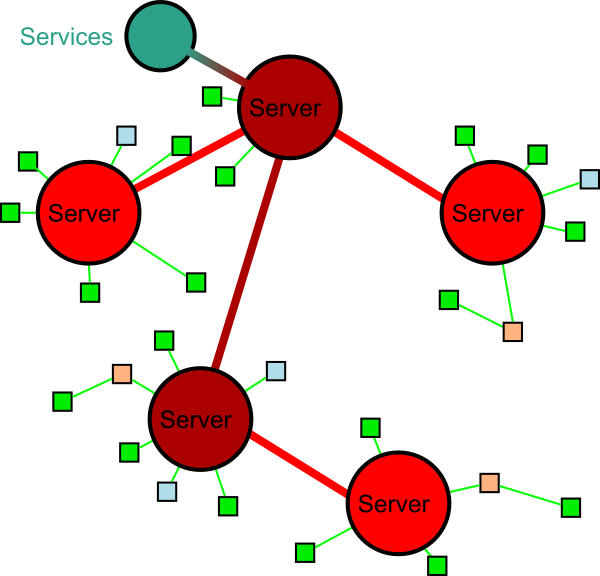
\includegraphics[width=0.7\linewidth]{Ircnetz.png}
  \caption{Schematischer Aufbau eines IRC-Netzes.}
  \label{abb:Ircnetz}
\end{figure}


\documentclass[12pt,a4paper]{article}
\usepackage[ngerman]{babel}
\usepackage{graphicx}{\tiny }

\begin{document}


\section{SourceForge}

\begin{figure}[h]
\centering

\includegraphics[width=0.5\linewidth]{sourceforge-logo}
\end{figure}

\subsection{Allgemeines}

SourceForge ist eigentlich ein englisches Wort und bedeutet soviel wie "´Quellentextschmiede"'. Es ist ein Repository in Form einer Website. Mit SourceForge ist es m\"oglich Softwareprojekte online zu erstellen und zu verwalten. Was dabei zu beachten ist, ist, dass eine Registrierung optional ist. Dass bedeutet, man kann \"offentliche Projekte auch ohne einen Account einsehen. SourceForge wird betrieben vom US-amerikanischen Unternehmen "`Dice Holdings"'. Au{\ss}erdem war es bis zur Version 3 eine freie Software, wurde daraufhin allerdings propriet\"ar und kommerziell vertrieben. Viele bekannte Open Source Projekte sind auf SourceForge vertreten, wie zum Beispiel Hibernate, Moodle oder auch FileZilla. Des Weiteren bietet SourceForge im Gegensatz zu vielen Konkurrenten, mehr als nur ein System zur Versionsverwaltung an. 

Dazu z\"ahlen: 
\begin{itemize}
	\item CVS
	\item SVN
	\item Bazaar
	\item Git
	\item Mercurial
\end{itemize}

SourceForge wird von vielen Software Entwicklern genutzt, weil es neben der Hauptaufgabe als Online-Repository noch weitere Vorteile bietet. Beispielsweise kann jedes Projekt \"uber ein eigenes Wiki verf\"ugen, in dem wichtige Informationen \"uber das Projekt aufgelistet sind. Ein anderer Punkt ist, dass SourceForge f\"ur jedes einzelne Projekt auch die M\"oglichkeit bietet, auf eine eigene MySQL-Datenbank zuzugreifen.

\subsection{Einschr\"ankungen}
Der Zugriff auf SourceForge wurde vor einiger Zeit in China gesperrt, aufgrund des Projektes "´Goldener Schild"'. Das soll eine Anlehnung an die Chinesische Mauer sein. Dieses Projekt ist f\"ur die \"Uberwachung der Zensur im chinesischen Internetverkehr zust\"andig. Allerdings wurde diese Sperrung nach bereits einem Jahr wieder aufgehoben. 2008 wurde der Zugang aber wieder gesperrt, weil vermutet wird, dass sich ein SourceForge-Programmierer negativ \"uber die chinesische Regierung ge\"au{\ss}ert hat. 

Des Weiteren wurde SourceForge in einigen sogenannten "´Schurkenstaaten"' gesperrt. Das sind Staaten, die auf der Sanktionsliste der USA sind. Einige betroffene Länder sind Nordkorea, Syrien, Sudan und Kuba. Aufgrund der Reaktion der Community wurde diese Einschränkung aber ein wenig gelockert. Es ist nun möglich, dass der Administrator jedes Projektes selbst bestimmen kann, ob er den Zugang zum Projekt in diesen Ländern freigeben möchte. 

\subsection{Kritikpunkte}
In letzter Zeit wurde SourceForge stark kritisiert, weil sie auf sogenannte "´Drive-By-Installer"' zurückgriffen. Diese sorgen daf\"ur, dass bei der Installation von SourceForge weitere Installationen von Adware von Drittanbietern vorgeschlagen wird. Ein Beispiel für eine solche Adware ist die "´Ask-Toolbar"'. Das ganze wurde wahrscheinlich gemacht, um an zus\"atzliches Geld zu kommen, allerdings war die Community damit nicht zufrieden und deswegen hat SourceForge in letzter Zeit stark an aktiven Mitgliedern verloren. 

\subsection{\"Ahnliche Projekte}

SourceForge war eine Art Vorreiter auf dem Gebiet von Online-Repositories. Heute gibt es allerdings jede Menge Konkurrenten, die teilweise auch schon erfolgreicher sind als SourceForge. Dazu zählt Github, ein Online-Repository, dass mit dem Versionsverwaltungssystem Git arbeitet. Weitere Beispiele sind Bitbucket, dass Mercurial zur Versionsverwaltung benutzt, Codeplex, was eine Hosting Website von Microsoft für Open Source Projekte ist und Freecode, ein Katalog für Open Source Projekte.

\end{document}

\section{Mercurial}
\begin{figure}[h]
  \centering
  
\includegraphics[scale=0.5]{logo-mercurial.png}
  \caption{Logo von Mercurial}
  \label{fig:mercurial}
\end{figure}
\noindent Mercurial ist ein verteiltes, programmunabhängiges Versionskontrollsystem.
\subsection{Geschichte}
Angekündigt wurde es von Matt Mackall auf der Linux-Kernel-Mailingliste am 19. April 2005. Diese Ankündigung war die Folge, dass die Firma BitMover, die z. B. für den Linux-Kernel als Versionskontrollsystem eingesetzte Software BitKeeper nicht mehr in einer kostenlosen Version bereitstellte. Zur selben Zeit startete Linus Torvalds das Projekt Git, das sich in der Folgezeit besser etablieren konnte als Mercurial.
\subsection{Implementierung}
Es ist nahezu in vollständig in Python entwickelt, weshalb es nicht unbedingt empfehlenswert wäre, Mercurial zu benutzen. Lediglich eine diff-Imple-mentierung, die mit binären Dateien umgehen kann, ist in C entwickelt, da das in Python nicht möglich ist. Nichtsdestotrotz sind Effizienz, Skalierbarkeit und robuste Handhabung von Text- und Binärdateien einige Punkte, die bei der Entwicklung als Schwerpunkte festgelegt wurden.

Ähnlich wie Git ist Mercurial kein zentralisiertes Versionskontrollsystem, d.h. man kann ein Repository klonen kann und auf einer lokalen Kopie darauf arbeiten. Auf dieser Kopie kann man ganz normal auf den die Funktionen von Mercurial verwenden. Ebenso ist die Fähigkeit des Erstellens und Zusammenfügens von Entwicklungszweigen ein fester Bestandteil dieses Versionskontrollsystems. Des Weiteren kann man einfach und schnell Unterschiede zwischen zwei unterschiedlichen Versionen anzeigen lassen. Zudem ist es möglich bei der Version Sekunden anzugeben, die man zurückspringen will.
\subsection{Zugriff}
Man kann sowohl über eine grafische Oberfläche als auch über die Komandozeile auf die Funktionen von Mercurial zugreifen. Eine grafische Oberfläche wird häufig bei Microsoft Windows, Gnome/Nautilus (jeweils TortoiseHg) und bei Mac OS X (MacHg und Murky). Bei gängigen Entwicklungsumgebungen wie Netbeans, Eclipse, Android Studio oder der Qt Creator erlauben es, ein externes Plugin zu installieren und das User-Interface der Entwicklungsumgebung ist es möglich, auf die Funktionen von Mercurial zuzugreifen.
\subsubsection{Terminal}
Über die Kommandozeile kann man über folgende Befehle auf Mercurial zugreifen:
\begin{itemize}
\item\textbf{Clonen}: hg clone \(<\)URL\(>\)
\item\textbf{Dateien hinzufügen}: hg add \(<\)Datei\(>\)
\item\textbf{Änderung}: hg revert \(<\)Datei\(>\)
\item\textbf{Änderungen bestätigen}: hg commit -m \(<\)Änderungstext\(>\)
\item\textbf{Repository auf den aktuellen Stand bringen}: hg update
\item\textbf{Branch mischen}: hg merge
\item\textbf{Versionsgeschichte des Repository erkunden}: hg log -v
\end{itemize}
Wie beim bereits im Unterricht behandelten GIT, muss man bei der Bestäti-gung von Änderungen eine Beschreibung der Änderung anfügen. Wenn das automatische Mischen nicht gelingt, muss man manuell die Konflikte lösen.
\subsection{Anwendungs-Beispiele}
Einige namhafte Firmen haben und bei bekannten Projekten wurde Mercurial eingesetzt. Dazu gehören Facebook, Mozilla (Firefox, Thunderbird), SourceForge, Google Inc. (Google Chrome, Google Code), Atlassian (Bitbucket), Microsoft (Codeplex), Oracle (OpenJDK), Xen, NetBeans IDE, Python und ClearCanvas.
\subsection{Fazit}
Zusammenfassend kann man sagen, dass Mercurial ähnlich dem Versionskontrollsystem Git ist, es gibt keine signifikante Unterschiede. Der größte Unterschied zwischen beiden Systemen ist der Performanceverlust durch den Python-Interpreter, weshalb es besser ist, Git als Versionskontrollsystem zu verwenden.

\section{Bitbucket}
    
	Bitbucket ist ein webbasierter Hosting-Dienst für Software-Entwicklungsprojekte, der die Versionsverwaltungssysteme Git und Mercurial unterstützt.
    
	\subsection{Geschichte}

		Der Dienst wurde ursprünglich als reines Mercurial-System von Jesper Nøhr entwickelt und 2010 von dem australischen Unternehmen Atlassian gekauft und am 3. Oktober 2011 um Unterstützung für Git erweitert.
    
	\subsection{Eigenschaften}
    
		In Bitbucket wir nicht das Projekt als Sammlung von Quelltexten verwaltet, sondern die Repositorys der Nutzer. Gleichzeitig wird das Erstellen (Branchen) und Wiedervereinigen (Mergen) von Abspaltungen (Forks) besonders propagiert. Bei Bitbucket ist es wie gesagt möglich, den eigenen Code zentral zu verwalten und zu versionieren. Dabei stehen zwei Versionierungs-Plattformen für die eigenen Repositories zur Verfügung: Git und Mercurial. Zusätzlich ist auch das Folgen von anderen Bitbucket-Nutzern und Teams möglich.

Bitbucket ist ein Web-basierter Online-Dienst, d.h. er läuft auf einem Browser und damit überall. Die Repositories befüllt man wie gehabt mit Git oder Mercurial von einem lokalen System aus. Bitbucket bietet zudem dank einer API auch verschiedene Apps an. Auf Android existiert beispielsweise die App Bitbeaker.

	\subsection{Kosten}

		Bitbucket hat ein Premium-Modell. Die Basis-Nutzung ist kostenlos. Diese Basis-Nutzung umfasst eine beliebe Anzahl an öffentlichen und privaten Repositories mit allen dazu nötigen Features, wie Issues, Wikis etc. Teams können aus bis zu 5 Mitgliedern bestehen, welche sich Repositories teilen. Diese Anzahl kann man bis auf 8 Mitglieder erhöhen. Wer mehr Mitglieder in seinem Team verwalten möchte, muss den Dienst bezahlen. Bei 10 Nutzern sind es 10\$/Monat, bei 25 Nutzern sind 25\$/Monat usw. Beim Unlimited-Plan bezahlt man 200\$/Monat.
	\subsection{Bitbucket vs Github}

		\begin{itemize}

			\item Bitbuckets offensichtlichster Vorteil ist die Möglichkeit, kostenlos eine unbegrenzte Zahl an privaten Repositories mit bis zu fünf Beteiligten zu hosten.

			\item Bitbucket unterstützt nicht nur Git sondern auch Mercurial.
			\item In Github ist es möglich öffentliche kostenlose Repositorys zu erstellen.

		\end{itemize}
	\subsection{Verwendungen}
		2014 arbeiteten über 330.000 Teams aus über 2,5 Millionen Entwicklern mit Bitbucket, 200 Terabyte Code wurden gehostet. Zu den Unternehmen, die Gebrauch von Bitbucket machen, zählen neben Atlassian:
		\begin{itemize}
			\item DHL
			\item PayPal
 
			\item Teslaa Motos
			\item The New Yorks Times
		\end{itemize}
Auch die Open-Source-Projekte Eigen und OGRE sind bei Bitbucket gehostet.
	\subsection{Fazit}
    
		Bitbucket ist ein webbasierter Hosting-Dienst wie Github. Im grunde genommen ergänzen sich die beiden Programme jedoch recht gut, den bei Bitbucket kann man unbegrenzt viele private Repositorys erstellen und bei Github hingegen kann man unbegrenzt viele öffentliche Repositorys erstellen.


\end{sloppypar}
\end{document}
